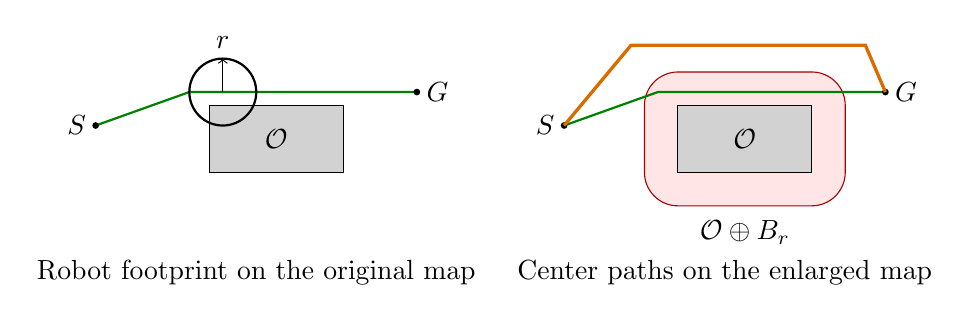
\begin{tikzpicture}[scale=.85]
\foreach \dx in {0,7} {
\begin{scope}[shift={(\dx,0)}]
\ifnum\dx=7
\filldraw[fill=red!10,draw=red!65!black] (2,0.5)--(4,.5) arc(-90:0:.5)--(4.5,2) arc(0:90:.5)--(2,2.5) arc(90:180:.5)--(1.5,1) arc(180:270:.5)--cycle;
\fi
\filldraw[fill=gray!35] (2,1) rectangle (4,2);
\draw[thick,green!50!black] (.3,1.7)--(1.7,2.2)--(5.1,2.2);
\fill (.3,1.7) circle(.05) node[left] {$S$};
\fill (5.1,2.2) circle(.05) node[right] {$G$};
\ifnum\dx=0
\draw[thick] (2.2,2.2) circle(.5);
\draw[->] (2.2,2.2)--(2.2,2.7) node[above] {$r$};
\node at (3,1.5) {$\mathcal O$};
\else
\draw[very thick,orange!85!black] (.3,1.7)--(1.3,2.9)--(4.8,2.9)--(5.1,2.2);
\node at (3,1.5) {$\mathcal O$};
\node at (3,.1) {$\mathcal O\oplus B_r$};
\fi
\end{scope}}
\node at (2.7,-.5) {Robot footprint on the original map};
\node at (9.7,-.5) {Center paths on the enlarged map};
\end{tikzpicture}
